\documentclass{article}
\usepackage[margin=2pt]{geometry}
\pagestyle{empty}
\usepackage{tikz}
\usetikzlibrary{arrows.meta,positioning}
\usepackage{helvet}
\renewcommand{\familydefault}{\sfdefault}
\usepackage[T1]{fontenc}
\definecolor{ikvblue}{HTML}{2F6DB3}
\definecolor{ikvnavy}{HTML}{1B4F8A}
\definecolor{ikvteal}{HTML}{5BB3A7}
\definecolor{ikvorange}{HTML}{D96B2B}
\definecolor{ikvgray}{HTML}{6B6B6B}
\begin{document}
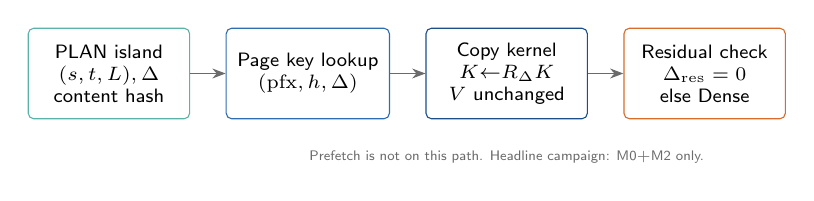
\begin{tikzpicture}[
  font=\sffamily\scriptsize,
  >=Stealth,
  box/.style={draw=#1, fill=white, rounded corners=2pt, align=center,
    minimum width=2.05cm, minimum height=1.15cm, inner sep=4pt},
]
\node[box=ikvteal] (a) {PLAN island\\$(s,t,L),\Delta$\\content hash};
\node[box=ikvblue, right=0.45cm of a] (b) {Page key lookup\\$(\mathrm{pfx}, h, \Delta)$};
\node[box=ikvnavy, right=0.45cm of b] (c) {Copy kernel\\$K{\leftarrow}R_{\Delta}K$\\$V$ unchanged};
\node[box=ikvorange, right=0.45cm of c] (d) {Residual check\\$\Delta_{\mathrm{res}}=0$\\else Dense};
\draw[->, ikvgray] (a) -- (b);
\draw[->, ikvgray] (b) -- (c);
\draw[->, ikvgray] (c) -- (d);
\node[font=\sffamily\tiny, text=ikvgray, below=0.28cm of c] {Prefetch is not on this path. Headline campaign: M0$+$M2 only.};
\end{tikzpicture}
\end{document}
